\documentclass[article,nojss]{jss}

\usepackage{inconsolata,amssymb,amsmath,xspace,bm,subfigure,graphicx}
\usepackage[authoryear,round]{natbib}
\usepackage{tikz,verbatim}
\usetikzlibrary{shapes,arrows}

%%%%%%%%%%%%%%%%%%%%%%%%%%%%%%
%% declarations for jss.cls %%%%%%%%%%%%%%%%%%%%%%%%%%%%%%%%%%%%%%%%%%
%%%%%%%%%%%%%%%%%%%%%%%%%%%%%%

%% almost as usual
\author{Gianluca Baio\\University College London}
\title{\pkg{survHE}: Survival analysis for health economic evaluation and cost-effectiveness modelling}

%% for pretty printing and a nice hypersummary also set:
\Plainauthor{Gianluca Baio} %% comma-separated
\Plaintitle{\pkg{survHE}: Survival analysis for health economic evaluation and cost-effectiveness modelling} %% without formatting
\Shorttitle{\pkg{survHE}: Survival analysis for health economics} %% a short title (if necessary)

%% an abstract and keywords
\Abstract{
  The abstract of the article.
}
\Keywords{Survival analysis, health economic evaluation, Probabilistic Sensitivity Analysis,~\proglang{R}}
\Plainkeywords{Survival analysis, health economic evaluation, Probabilistic Sensitivity Analysis,~R} %% without formatting
%% at least one keyword must be supplied

%% publication information
%% NOTE: Typically, this can be left commented and will be filled out by the technical editor
%% \Volume{50}
%% \Issue{9}
%% \Month{June}
%% \Year{2012}
%% \Submitdate{2012-06-04}
%% \Acceptdate{2012-06-04}

%% The address of (at least) one author should be given
%% in the following format:
\Address{
  Gianluca Baio\\
  Department of Statistical Science\\
  University College London\\
  Gower Street, London, WC1E 6BT (UK)\\
  E-mail: \email{g.baio@ucl.ac.uk}\\
  URL: \url{http://www.statistica.it/gianluca}
}
%% It is also possible to add a telephone and fax number
%% before the e-mail in the following format:
%% Telephone: +43/512/507-7103
%% Fax: +43/512/507-2851

%% for those who use Sweave please include the following line (with % symbols):
%% need no \usepackage{Sweave.sty}

%% MY COMMANDS
\newcommand{\ie}{{\em i.e.\/}\xspace}
\newcommand{\eg}{{\em e.g.\/}\xspace}
\newcommand{\R}{\proglang{R}\xspace}
\newcommand{\sh}{\proglang{survHE}\xspace}
\newcommand{\fs}{\proglang{flexsurv}\xspace}
\newcommand{\INLA}{\proglang{INLA}\xspace}
\newcommand{\ob}{\proglang{R2OpenBUGS}\xspace}
\newcommand{\bugs}{\proglang{OpenBUGS}\xspace}

\begin{document}
\section{Introduction}
Health economic modelling is often focussed on data on survival. That is typically the case when using multistate structures (commonly referred to as ``Markov models'' in the health economics literature), for example in the case of modelling for interventions aimed at treating cancer. In those cases, the model would comprise of a set of relevant clinical states (\eg \textit{Pre-progression}, \textit{Post-progression}, \textit{Death}). Figure \ref{MM} shows a possible graphical representation for this simple model: the three states are connected by arrows, indicating the possibility that from one time point to the next, patients may \textit{transition} from the state from which the arrow originates to the one reached by it.

\begin{figure}[!h]
\centering
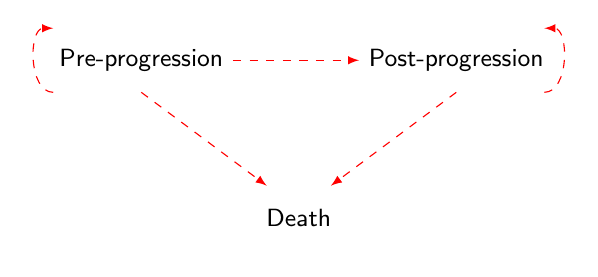
\begin{tikzpicture}
\draw(-2,2) node[align=center,draw=none,fill=none,minimum width=.4cm,minimum height=.8cm,font=\sffamily\fontsize{9}{10}\selectfont](1){Pre-progression};
\draw(2,2) node[align=center,draw=none,fill=none,minimum width=.4cm,minimum height=.8cm,font=\sffamily\fontsize{9}{10}\selectfont](2){Post-progression};
\draw(0,0) node[align=center,draw=none,fill=none,minimum width=.4cm,minimum height=.8cm,font=\sffamily\fontsize{9}{10}\selectfont](3){Death};

\draw [dashed,->,>=latex,shorten >=0pt,auto,node distance=0cm,thin,color=red] (1.200) to [bend left=90] (1.160);
\draw [dashed,->,>=latex,shorten >=0pt,auto,node distance=0cm,thin,color=red] (2.340) to [bend left=-90] (2.20);
\draw [dashed,->,>=latex,auto,node distance=0cm,thin,color=red] (1.east) -- (2.west);
\draw [dashed,->,>=latex,shorten >=0pt,auto,node distance=0cm,thin,color=red] (1.south) -- (3.135);
\draw [dashed,->,>=latex,shorten >=0pt,auto,node distance=0cm,thin,color=red] (2.south) -- (3.45);
\end{tikzpicture}
\caption{An example of Markov model for a fictional cancer problem}\label{MM}
\end{figure}

Often, the transition probabilities $\pi_{rs}$ that govern the movement of individuals from state $r$ to state $s$ in the Markov model are estimated using survival data, \ie obtained from a (possibly small) randomised clinical trial, with usually a limited follow up.  In addition, economic model is concerned with the long-term modelling of the benefits and costs associated with a health care intervention, \eg the introduction of a new drug on the market. For this reason, it is usually necessary to \textit{extrapolate} the results obtained from the trial to a (much) longer follow up time. For example, we may be interested in evaluating the economic performance of a new proposed intervention over the course of several years, despite the fact that the follow up from the trial may only cover 12 months.

One important consequence is that unlike in standard biostatistical analysis (where non- or semi-parametric models, such as the Cox Proportional Hazards model are usually applied), modelling in health economics is typically based on \textit{parametric} models, which allows relatively straightforward calculation of the mean survival time. This is the actual quantity of interest when it comes to \textit{extrapolating} the survival curves beyond the observed data.

The guidelines in the health economics literature suggest that the modeller assesses the impact of the parametric model chosen for the survival data and produces a comprehensive sensitivity analysis. This is particularly relevant as the objective of health economic evaluation is not a statistical analysis \textit{per se}; rather, this is used to feed into an economic model, which is used to make a decision over the possible therapeutic options.

\section{The R package survHE}
\sh is an \R package specifically designed to aid in the process of survival analysis for health economic evaluation and cost-effectiveness analysis. In fact, \sh can be actually considered as a wrapper for some other \R packages; the first one, \fs, is in turn a general-purpose tool for performing several types of survival analysis using maximum likelihood estimates (MLEs). The second, \ob is a \R package that can be used to interface \R and \bugs, probably the most popular engine for Bayesian computation using Markov Chain Monte Carlo (MCMC); and the third one, \INLA can be used to perform fast Bayesian computations (on a limited set of survival models) using Integrated Nested Laplace Approximation. In a sense, thus, \sh is a very simple package that specialises functions from other relevant packages and builds some other specific commands to simplify and standardise the process of using survival data in health economic evaluation.

As a first example, suppose that the user has a suitable dataset, perhaps obtained from a trial, in which data are recorded for the time at which observations are made, a censoring indicator taking value 0 if an event (\eg progression to a cancerous state, or death) has actually occurred at that time and 1 if the individual has been censored (\eg we have not observed any event at the end of follow up) and an arm indicator, specifying whether the individual to which the data refer belongs in the control or the active treatment arm of the trial. Of course, other variables may be observed (\eg as relevant covariates, such as sex, age, co-morbidity). 

For the moment we consider the simple case in which the data are available in the \R workspace as a data frame (say, \code{data}) that can be partially visualised using the following command:
\begin{CodeInput}
rbind(head(data),tail(data))
\end{CodeInput}
to show the first 6 and the last 6 rows:
\begin{CodeOutput}
   ID_patient  time censored arm
1            1  0.03        0   0
2            2  0.03        0   0
3            3  0.92        0   0
4            4  1.48        0   0
5            5  1.64        0   0
6            6  1.64        0   0
362        362 13.97        1   1
363        363 14.56        1   1
364        364 14.56        1   1
365        365 14.85        1   1
366        366 16.07        1   1
367        367 18.16        1   1
\end{CodeOutput}
In this case, the dataset consists of 367 individuals in total, grouped in two arms (here \code{arm} = 0 indicates the controls and \code{arm} = 1 indicates the active treatment).

\subsection{Model fitting: to be or not to be (Bayesian)?...}
By relying on either \fs, \INLA or \ob and \bugs, \sh can fit models under the frequentist or Bayesian framework. 

In general terms, a Bayesian approach has several advantages: for example, health economic evaluations are typically based on complex models, often made by several (correlated) modules, which may be informed by different and diverse sources of evidence. Thus, a Bayesian approach can be beneficial to propagate the underlying uncertainty in all the model parameters in a principled way. This is also particularly relevant in terms of what is often termed in ``probabilistic sensitivity analysis'' (PSA) in health economics. That is the practice of assessing the impact of parameters uncertainty on the decision-making process and is usually based on a simulation approach to characterise the underlying uncertainty in the model parameters --- a fundamentally Bayesian operation.

On the other hand, Bayesian models for survival analysis fitted using MCMC can be computationally intensive and sometimes have problems with convergence; perhaps for this reason, often practitioners use MLE-based routines to obtain relevant estimates from the survival component of the wider economic model. These are usually simple to obtain. In order to deal with PSA, \fs uses bootstrap (based on multivariate Normal distributions), which may be a good approximation of the underlying full joint posterior distribution of the survival parameters.

A good compromise is provided by \INLA, which is effectively an alternative method of performing Bayesian inference. Typically, \INLA requires a computational time that is very close to that of MLE-based routines, while also estimating a full joint posterior distribution for the model parameters. However, in general terms, it is a bit more complex to embed \INLA within a more complex model; in addition, currently, \INLA can only fit a limited number of survival~models. 

For these reasons, we chose to design \sh around these three approaches: ideally, we would build the whole economic model under a Bayesian framework and take full advantage of the flexibility provided by MCMC estimation --- this would be naturally obtained by using \ob and \bugs. However, we acknoledge that at times it may be helpful to fit Bayesian survival models separately and \INLA is very helpful (for the range of distributions it supports); similarly, some practitioners (particularly in specific settings) may want to use a standard approach to statistical inference and MLEs. 

The combined use of \sh and its ``dependencies'' (in the \R parlance) allows all of these options in a unified framework. More importantly, irrespective of the way in which the inference on the survival model is performed, \sh has a set of built-in functions that can be used to produce a standardised post-processing of the results, for their inclusion in the economic model and PSA.

\subsection{Modelling framework}
The general modelling framework considered in \sh can be described as follows. The observed data are at least made by the pair $(t_i,d_i)$, for $i=1,\ldots,n$, where $t_i>0$ is the observed time at which the event under study occurs and $d_i$ (for ``dummy'' variable) is an event indicator, taking value 1 if the event actually happens (in which case $t_i$ is indeed observed), or 0 when the $i-$th individual is ``censored''. In this latter case, we do not know whether the event actually occurs --- it may in the future, but we just do not have this information. Consequently, when $d_i=0$, then $t_i$ is missing.

The observed data are modelled using a suitable probability distribution $t_i \sim f(t_i\mid \bm\theta)$, as a function of a vector of relevant parameters $\bm\theta$. This can be linked to the \textit{survival function} 
\[ S(t) = 1-F(t) = 1 - \int_0^u f(u\mid\bm\theta)du, \]
indicating the probability of an individual surviving up to time $t$ and the \textit{hazard function}
\[ h(t) = \frac{f(t)}{S(t)}, \]
which quantifies the instantaneous risk of experiencing the event. In the presence of censoring, the resulting likelihood function is modified to account for the possibility of missing data (in correspondence with censoring)
\[ \mathcal{L}(\bm\theta) = \prod_{i=1}^n h(t_i)^{d_i}S(t_i). \]
This basically models the risk of experiencing the event at any time point $t$, conditionally on the fact that the $i-$th unit has in fact survived up to that time point (if they have not, then the probability of experiencing the event again is 0).

When formulating a parametric survival model, we need to specify the form of the probability distribution assumed to describe the underlying uncertainty in the observed times. As mentioned above, it is good practice to test a set of (more or less) plausible parametric models for the survival data. 

In general terms, we can specify the vector of relevant parameters as $\bm\theta=\left(\mu(\bm{x}),\alpha(\bm{x})\right)$. In this notation, we consider: a vector of potential covariates $\bm{x}$ (\eg age, sex, trial arm, etc.); a \textit{location} parameter $\mu(\bm{x})$, which indicates the mean or the scale of the probability distribution; and a (set of) ancillary parameter(s) $\alpha(\bm{x})$, which describes the shape or variance of the distribution. While it is possible for both $\mu$ and $\alpha$ to explicitly depend on the covariates $\bm{x}$, usually the formulation is simplified to assume that these only affect directly the location parameter.

In addition, since $t>0$, we typically use a generalised linear model in the form
\begin{eqnarray} 
g(\mu_i) = \beta_0 + \sum_{j=1}^J \beta_j x_{ij} [+ \ldots]  \label{linpred}
\end{eqnarray}
to model the location parameter. The function $g(\cdot)$ is typically the logarithm (notice that here we slightly abuse the notation and omit the dependence on $\bm{x}$). Generally speaking, (\ref{linpred}) can be extended to include additional terms --- for instance, we may want to include random effects to account for repeated measurements or clustering. We indicate this possibility using the $[+ \ldots]$ notation.

The objective of the statistical analysis is the estimation of the parameters $\bm\theta$, which can then be used to obtain estimates for all the relevant quantities (\eg the survival function), which are then in turn used in the economic modelling (\eg to estimate the transition probabilities in a Markov model).

In a frequentist setting, the estimation procedure concerns some relevant statistics (\ie functions of the observed data). The estimation is obtained via maximum likelihood estimation. Conversely, in a full Bayesian setting, the parameters are directly modelled using a prior probability distribution, which is updated by the observed data into a posterior. It is this posterior distribution that is the object of the inferential process. Thus, when using a Bayesian framework, the model needs to be completed by specifying suitable prior distributions for the parameters $\bm\theta$.

Assuming that the location parameter is specified using a log-linear predictor form
\[\log(\mu_i) = \beta_0 + \sum_{j=1}^J \beta_j x_{ij}, \]
as a function of $J$ covariates, we can model $\bm\beta = (\beta_0,\beta_1,\ldots,\beta_J) \stackrel{iid}{\sim}\mbox{Normal}(0,v)$, where $v$ is a large constant. This amounts to specifying a ``minimally informative'' prior on the regression coefficients that determine the location parameter --- in other words, we are not including strong prior information in this aspect of our model. The observed data (and the censoring structure) will be mainly driving the update to the posterior distribution. 

As for the ancillary parameter, the choice of prior depends on the specification of the probability distribution selected to model the observed data. Table \ref{Models} shows a summary of the models directly implemented in \sh. In each, by default we specify minimally informative priors on the relevant parameters; for example, in the Weibull model, we define $\alpha\sim\mbox{Gamma}(a,b)$, for given values of $a,b$. This is of course just a simplification and genuine information should be included in the model, when available. We return to this point in \S\ref{model_inla}-\ref{model_bugs}.

\begin{table}[!h]
\fontsize{7}{9.5}\selectfont
\centering
\begin{tabular}{p{.21\textwidth}p{.31\textwidth}p{.21\textwidth}p{.18\textwidth}}
\hline
Data model & Location parameter & Ancillary parameter & Survival function $S(t)$ \\
\hline
$t_i \sim \mbox{Exponential}(\mu_i)$ & Rate: $\mu_i$;\par Scale: $\displaystyle\lambda_i = \frac{1}{\exp(\beta_0 + \sum_{j=1}^J \beta_jx_{ij})}$ & $-$ & $\displaystyle\exp\left(-t/\lambda_i \right)$ \\[1.2cm]
$t_i \sim \mbox{Weibull}(\mu_i,\alpha)$ & Mean: $\mu_i$;\par Scale: $\displaystyle\lambda_i\!=\!\exp\left(\beta_0 + \sum_{j=1}^J \beta_jx_{ij}\right)^{\frac{1}{-\alpha}}$ & Shape: $\alpha \sim \mbox{Gamma}(a,b)$ & $ \displaystyle\exp\left( -(t/\lambda_i)^\alpha \right) $\\[1.2cm]
$t_i \!\sim\! \mbox{Gen Gamma}(1, \mu_i,\alpha)$ & Mean: $\mu_i$;\par Scale: $\displaystyle\lambda_i\!=\!\exp\left[- \left( \beta_0 + \sum_{j=1}^J \beta_j x_{ij} \right)\right]$ & Shape: $\alpha \sim \mbox{Gamma}(a,b)$ & $ \displaystyle\exp\left( -(t/\lambda_i)^\alpha \right) $\\[1.2cm]
$t_i \sim \mbox{logNormal}(\mu_i,\alpha^2)$ & Mean: $\mu_i$ & log-sd: $\alpha \sim \mbox{Uniform}(0,k)$ & $\displaystyle 1- \Phi\left( \frac{\log(t)-\mu}{\alpha} \right)$ \\[1.2cm]
$\log(t_i) \sim \mbox{Logistic}(\mu_i,\tau)$ & Mean: $\mu_i$;\par Scale: $\displaystyle\lambda_i\!=\!\exp\left[- \left( \beta_0 + \sum_{j=1}^J \beta_j x_{ij} \right)\right]$ & Shape: $\tau=\alpha^{-2}$;\par log-sd: $\alpha\sim\mbox{Uniform}(0,k)$ & $\displaystyle\frac{1}{1+(t/\lambda_i)^{\tau}}$\\[1.2cm]
\hline
\end{tabular}
\caption{}\label{Models}
\end{table}



\subsection{MLE via flexsurv}
When using MLE routines to fit the models, \sh allows the user to define in \R a vector of model names (in the format that \fs can recognise). We could for instance decide that we want to consider the Exponential, Weibull, Gamma, logNormal, logLogistic and Generalised Gamma models for our analysis (other choices are possible, but for now we concentrate on this fairly wide range).

We can do this in \R by using the following commands.
\begin{CodeInput}
mods <- c("exp","weibull","gamma","lnorm","llogis","gengamma")   
\end{CodeInput}
%n.mods <- length(mods)
%colors <- seq(2,(n.mods+1))
%labs <- c("Exponential","Weibull","Gamma","log-Normal","log-Logistic",
%	"Generalised Gamma")
This syntax defines a vector of model names to be used by \fs in the fitting process. These \textit{must} adhere with \fs convention.
%; colors, to distinguish the survival curves (in the \R notation the numbers in the sequence spanning from 2 to the number of models used incremented by 1, for reasons that will become clear later); and model labels, which effectively describe the model names in human-readable terms. While the elements of the vector \code{mods} \textit{must} adhere with \fs convention, the labels can be specified in any way the user wants (so, for instance we could have typed \code{lognormal}, instead of \code{log-Normal}).
At this point, we are almost ready to actually perform the survival analysis using the 6 models specified above; before we can do this, however, we need to specify the model ``formula''
\begin{CodeInput}
formula <- as.formula("Surv(time, censored) ~ as.factor(arm)")
\end{CodeInput}
This creates an object instructing \R to analyse the data using a survival model in which the only covariate is the treatment arm, interpreted as an \R ``factor'' (\ie a categorical variable).

The \sh function \code{fit.models} can be used to actually perform this analysis in batch, \eg by typing the command
\begin{CodeInput}
fit.mle <- fit.models(formula=formula,data=data,distr=mods)
\end{CodeInput}
The function \code{fit.models} takes as mandatory inputs the analysis formula, the name of the dataset to be used and the type of distribution(s) to be fitted. Just like in this case, this may be a vector, in which case \code{fit.models} will store all the different analyses in the resulting object. This creates a list \code{fit} in which the results of the survival analyses are stored for each parametric model considered. The usual \R command
\begin{CodeInput}
names(fit)
\end{CodeInput}
returns the names of the list's elements:
\begin{CodeOutput}
[1] "models"        "model.fitting" "method"        "misc"         
\end{CodeOutput}
The object \code{models} is itself a list, in this case containing 6 elements (one for each of the parametric models fitted). For example, the first one can be accessed using the standard \R notation \code{fit$model[[1]]} %$
(\ie using ``double square brackets'') and can be inspected typing the command
\begin{CodeInput}
names(fit$model[[1]])
\end{CodeInput}
\begin{CodeOutput}
 [1]  "call"           "dlist"          "aux"            "ncovs"          
 [5]  "ncoveffs"       "mx"             "basepars"       "covpars"        
 [9]  "AIC"            "data"           "datameans"      "N"              
 [13] "events"         "trisk"          "concat.formula" "all.formulae"   
 [17] "dfns"           "res"            "res.t"          "cov"            
 [21] "coefficients"   "npars"          "fixedpars"      "optpars"        
 [25] "loglik"         "logliki"        "cl"             "opt"  
\end{CodeOutput}
%$
The quantities included in the model objects are the output from \fs. Typically, the user does not need to access or manipulate them directly (that is the point of \sh!); in fact, other \sh functions will use these to produce plots or further analyses. Users familiar with \R programming can however access them to post-process their results and customise the output provided by \sh.

%%%%%The results from each model can be easily shown by simply typing
%%%%%\fontsize{9}{10}\selectfont
%%%%%\begin{CodeInput}
%%%%%fit$models
%%%%%\end{CodeInput}
%%%%%\begin{CodeOutput}
%%%%%[[1]]
%%%%%Call:
%%%%%flexsurvreg(formula = formula, data = data, dist = distr[i])
%%%%%
%%%%%Estimates: 
%%%%%                 data mean  est       L95%      U95%      se        exp(est)  L95%      U95%    
%%%%%rate                   NA    0.08242   0.06768   0.10037   0.00828        NA        NA        NA
%%%%%as.factor(arm)1   0.48501   -0.46561  -0.76797  -0.16324   0.15427   0.62775   0.46395   0.84939
%%%%%
%%%%%N = 367,  Events: 172,  Censored: 195
%%%%%Total time at risk: 2612.07
%%%%%Log-likelihood = -635.2881, df = 2
%%%%%AIC = 1274.576
%%%%%
%%%%%
%%%%%[[2]]
%%%%%Call:
%%%%%flexsurvreg(formula = formula, data = data, dist = distr[i])
%%%%%
%%%%%Estimates: 
%%%%%                 data mean  est      L95%     U95%     se       exp(est)  L95%     U95%   
%%%%%shape                 NA     1.8164   1.6134   2.0449   0.1098       NA        NA       NA
%%%%%scale                 NA    10.2210   9.1617  11.4026   0.5705       NA        NA       NA
%%%%%as.factor(arm)1   0.4850     0.3420   0.1744   0.5097   0.0855   1.4078    1.1905   1.6648
%%%%%
%%%%%N = 367,  Events: 172,  Censored: 195
%%%%%Total time at risk: 2612.07
%%%%%Log-likelihood = -598.5649, df = 3
%%%%%AIC = 1203.13
%%%%%
%%%%%
%%%%%[[3]]
%%%%%Call:
%%%%%flexsurvreg(formula = formula, data = data, dist = distr[i])
%%%%%
%%%%%Estimates: 
%%%%%                 data mean  est      L95%     U95%     se       exp(est)  L95%     U95%   
%%%%%shape                 NA     2.4041   2.0028   2.8858   0.2240       NA        NA       NA
%%%%%rate                  NA     0.2540   0.1981   0.3256   0.0322       NA        NA       NA
%%%%%as.factor(arm)1   0.4850    -0.3514  -0.5299  -0.1729   0.0911   0.7037    0.5887   0.8412
%%%%%
%%%%%N = 367,  Events: 172,  Censored: 195
%%%%%Total time at risk: 2612.07
%%%%%Log-likelihood = -598.752, df = 3
%%%%%AIC = 1203.504
%%%%%
%%%%%
%%%%%[[4]]
%%%%%Call:
%%%%%flexsurvreg(formula = formula, data = data, dist = distr[i])
%%%%%
%%%%%Estimates: 
%%%%%                 data mean  est     L95%    U95%    se      exp(est)  L95%    U95%  
%%%%%meanlog              NA     2.0997  1.9604  2.2391  0.0711      NA        NA      NA
%%%%%sdlog                NA     0.8185  0.7340  0.9127  0.0455      NA        NA      NA
%%%%%as.factor(arm)1  0.4850     0.3445  0.1469  0.5420  0.1008  1.4113    1.1583  1.7195
%%%%%
%%%%%N = 367,  Events: 172,  Censored: 195
%%%%%Total time at risk: 2612.07
%%%%%Log-likelihood = -604.4921, df = 3
%%%%%AIC = 1214.984
%%%%%
%%%%%
%%%%%[[5]]
%%%%%Call:
%%%%%flexsurvreg(formula = formula, data = data, dist = distr[i])
%%%%%
%%%%%Estimates: 
%%%%%                 data mean  est     L95%    U95%    se      exp(est)  L95%    U95%  
%%%%%shape                NA     2.2337  1.9744  2.5271  0.1406      NA        NA      NA
%%%%%scale                NA     8.1609  7.1917  9.2607  0.5264      NA        NA      NA
%%%%%as.factor(arm)1  0.4850     0.3484  0.1634  0.5333  0.0944  1.4167    1.1775  1.7045
%%%%%
%%%%%N = 367,  Events: 172,  Censored: 195
%%%%%Total time at risk: 2612.07
%%%%%Log-likelihood = -601.2472, df = 3
%%%%%AIC = 1208.494
%%%%%
%%%%%
%%%%%[[6]]
%%%%%Call:
%%%%%flexsurvreg(formula = formula, data = data, dist = distr[i])
%%%%%
%%%%%Estimates: 
%%%%%                 data mean  est     L95%    U95%    se      exp(est)  L95%    U95%  
%%%%%mu                   NA     2.2918  2.1357  2.4479  0.0796      NA        NA      NA
%%%%%sigma                NA     0.5871  0.4613  0.7471  0.0722      NA        NA      NA
%%%%%Q                    NA     0.8507  0.3620  1.3394  0.2493      NA        NA      NA
%%%%%as.factor(arm)1  0.4850     0.3463  0.1743  0.5183  0.0878  1.4138    1.1904  1.6792
%%%%%
%%%%%N = 367,  Events: 172,  Censored: 195
%%%%%Total time at risk: 2612.07
%%%%%Log-likelihood = -598.3923, df = 4
%%%%%AIC = 1204.785
%%%%%\end{CodeOutput}
%%%%%%$
%%%%%\normalsize
%%%%%In this case the output is rather long as it involves 6 models. For each, the specific parameters are summarised, together with some general information on the raw data and the model fit (in terms of the log-likelihood and the AIC). 
%%%%%%Notice that \fs standardises the output table to include an estimate and confidence interval on the natural and the exponentiated scale; in cases where no transformation is required for the parameters (\eg in the case of \code{fit[[2]]}, which shows the results for the Weibull model), the exponentiated values are reported as \code{NA}.

The other elements of the object \code{fit} are: 
\begin{itemize}
\item \code{model.fitting}: a list storing some suitable statistics that can be used to assess, well, model fitting. These are the Akaike, Bayesian and Deviance Information Criteria (AIC, BIC and DIC, respectively). The former two can be estimated using both the Bayesian and frequentist approach, while the latter is specific to Bayesian modelling. Thus, in this case, the \R call 
\begin{CodeInput}
> fit.mle$model.fitting
\end{CodeInput} 
%$
will return the following results
\begin{CodeOutput}
$aic
[1] 1274.576 1203.130 1203.504 1214.984 1208.494 1204.785

$bic
[1] 1282.387 1214.846 1215.220 1226.700 1220.211 1220.406

$dic
NULL
\end{CodeOutput}
%$
--- note that because we are storing the results obtained from fitting 6 models in the same object, the elements \code{$aic} and \code{$bic} %$
are vectors. In general, the model associated with the lowest information criterion tends to be associated with a better fit.
\item \code{method}: a string describing the method used to fit the model(s). In this case the code
\begin{CodeInput}
> fit.mle$method
\end{CodeInput}
%$ 
returns the output
\begin{CodeOutput}
"mle"
\end{CodeOutput}
\item \code{misc}: a list containing some miscellanea --- these are mainly used internally by the other functions in \sh to do plots and tables or other calculations. 
\end{itemize}

\subsection{Full Bayesian analysis via R-INLA}\label{model_inla}
When fitting models using a Bayesian approach via \INLA, \sh allows the user to select a vector of distributions; currently, \INLA and its \R implementation allow four survival models: Exponential, Weibull, log-Normal and log-Logistic. The user can specify a vector \code{distr <- c("exp","weibull","lognormal","loglogistic")}, or select only one of those models and may be run the \code{fit.models} command separately for each of them. If a distribution is specified that is not allowed in \INLA, then \sh will fall back on the MLE.

One important distinction is in the way in which \fs and \INLA handle the names of the distributions to be fitted and the formula specifying the model. As for the former, the correct notation is the following: \code{"exponential"}, \code{"weibull"}, \code{"lognormal"} and \code{"loglogistic"} --- these do not directly match with the \fs notation mentioned above. To avoid issues, \sh recodes internally the names given to the distributions. Thus, if the user specifies the additional option \code{method="inla"} in the call to \code{fit.models}, then the string \code{"exp"} (which would be accepted by \fs) will be recoded to \code{"exponential"}, which is required by \INLA. Similarly if a distribution that is accepted by \fs is given by the user in \INLA terminology but the \code{method} is either unspecified or specifically set to \code{"mle"} in the call to \code{fit.models}, then \sh will recode the name of the distribution in \fs terms.

With regards to the model formula, \INLA requires that this is specified using the notation 
\begin{CodeInput}
> formula <- inla.surv(time,event) ~ ...
\end{CodeInput}
where \code{time} and \code{event} are the variables in which the times and the event indicator are saved and \code{...} is a suitable form for the combination of covariates to be used. Again, \sh tries to simplify the modeller's life by fixing the code provided for the formula, depending on the value specified for the option \code{method}. So if \code{method="inla"} but the formula is specified using the \fs terminology, \sh will recode this to make it acceptable to \INLA.

A suitable call to \code{fit.models} using \INLA is the following.
\begin{CodeInput}
> fit.inla <- fit.models(formula=formula,data=dat,distr=distr,method="inla") 
\end{CodeInput}
%,control.family=list(lognormal=list(initial=0)))
which will fit the four available models.

When \code{method} is set to \code{"inla"}, then other options become available to the call to \code{fit.models}, which allow the user to customise the underlying setting of the Bayesian model and inferential procedure. In particular, it is possible to add the following arguments.
\begin{itemize}
\item \code{dz}; this defines the step length for the grid search over the hyperparameters space (default = 0.1). In a nutshell, the \INLA procedure is based on a nested approximation, the first of which tries to estimate the value of the hyperparameters in the model (\eg the shape of a Weibull distribution), using a grid search. The finer this grid, the more accurate (but more computationally expensive!) the resulting estimates (for all the parameters, \eg for both the shape and scale of the Weibull distribution). 
\item \code{diff.logdens}; defines the difference in the log-density for the hyperparameters to stop integration (default = 5). Again, this is related to how the hyperparameters are estimated in the first stage of the nested algorithm. Decreasing this difference is likely to increase the computational time (since the estimation of the hyperparameters will become more accurate).
\item \code{control.fixed}; defines the default for the prior distributions, unless specified by the user. By default, \INLA assumes that ``fixed effects'' associated with covariates are modelled using a Normal with mean 0 and variance 1000, while the overall intercept is modelled using a Normal with 0 mean and even smaller precision.
\item \code{control.family}; a list of options controlling the model for the observed data. If \code{distr} is a vector, then this can be provided as a named list of options; for example something like: 
\begin{CodeInput}
> fit.inla <- fit.models(formula=formula,data=dat,distr=distr,method="inla",
+     control.family=list(
+                    weibull=list(param=c(.1,.1)),
+                    lognormal=list(initial=2)
+     )
)
\end{CodeInput}
would instruct \INLA to assume a Gamma$(0.1,0.1)$ prior distribution for the shape parameter of the Weibull model and to use an initial value of 2 for the approximation routine of the log-Normal model. Notice that in this case, the names of the elements of the list need to be the same as those given in the vector \code{distr}.
\end{itemize}

Using the \INLA advanced controls is very powerful and allows much flexibility in fitting the models. However, some knowledge and understanding of the \INLA syntax and philosophy is required. Guidance is provided in the \INLA help functions as well as, for example, in \cite{Rueetal:2008,Blangiardoetal:2013,BlangiardoCameletti:2015}.

\subsection{Full Bayesian analysis via OpenBUGS and R2OpenBUGS}\label{model_bugs}

\subsection{Visual interpretation}
By default, \code{fit.model} does not display a graphical summary of the model fitted, but this can be overruled by setting the option \code{plot=T}, which generates a graph like the one shown in Figure \ref{KM_models}.
\begin{figure}[!h]
\centering
\includegraphics{KM_models}
\caption{}\label{KM_models}
\end{figure}

This graph shows the Kaplan-Meier (KM) estimate from the original data in addition to the model-based survival curves for each of the models specified. For this reason, in the graph there are in fact \code{n.mods+1} curves --- and thus we have specified that the colouring scheme should range from the value `2' (which in \R indicates red) to the value `\code{n.mods+1}' (= 7, in this case, which in \R indicates yellow), implicitly reserving code 1 (black) for the KM estimate. Of course, the user can select a different colouring scheme, \eg by setting a vector of pre-determined colours. In addition to the KM estimates and their non-parametric 95\% interval Figure \ref{KM_models} also displays the estimated survival curves for each of the selected models. 

When the option \code{plot=T} is specified, \code{fit.model} will also ask interactively whether the user wants to automatically save the graph. 
\begin{CodeInput}
fit <- fit.models(formula,data,distr=mods,plot=T,
	labs=labs,colors=colors,lab.trt=c("Control","Active"))
\end{CodeInput}
\begin{CodeOutput}
Would you like to save the graph? 

1: yes
2: no

Selection:
\end{CodeOutput}
If the user selects \code{1}, then \sh will also ask for the format to which save the graph (options are \code{jpeg}, \code{pdf}, \code{bmp}, \code{png} and \code{tiff}) and will automatically store the resulting graph to a file named \code{Graph.ext} in the current directory (here \code{ext} is the selected extension for the file type).

In any case, \sh also contains another utility function that allows to reproduce the graph of Figure \ref{KM_models}, once the models have been fitted. This can be done using the command
\begin{CodeInput}
fit.plot(fit,labs=labs,colors=colors,lab.trt=c("Control","Active"))
\end{CodeInput}
The arguments to \code{fit.plot} are similar to the ones included directly in the call to \code{fit.models}, with the major exception that the first mandatory input is now the results of a call to \code{fit.models} --- in this case, the object named \code{fit}.

Other optional arguments allow the user to modify the aspect of the graph. These can be specified both in \code{fit.models} and \code{fit.plot} and are: the vector of model labels (\code{labs}); the vector of colours (\code{colors}); the vector of labels associated with the treatments (\code{lab.trt}) and the font size for the curves labels (\code{cex.trt}, which by default is set at 0.8 of the normal size). Notice that currently \sh considers only data with two treatment arms. 

The graph produced by \sh also shows the actual number of individuals who are still alive at each time interval, which can be used to describe the survival patterns; these can be turned off by setting the optional argument \code{n.risk=FALSE} in the call to either \code{fit.models} or \code{fit.plot}. It is possible to customise the labels for the $x-$ and $y-$ axis using standard \R notation, by specifying the options \code{xlab} and \code{ylab} --- the default values are respectively ``time'' and ``Survival''. Similarly, it is also possible to modify the range of the two axes in the graph, by simply setting the options \code{xlim=c(low.x,upp.x)} and \code{ylim=c(low.y,upp.y)}, where \code{low.x} and \code{low.y} represent the lower limit of the range for the $x-$ and $y-$ axis respectively; similarly, \code{upp.x} and \code{upp.y} determine the two upper limits. This can be useful to add a graphical representation of the extrapolated surival curves, as we will show later.

\subsection{Model assessment}
Health economic guidelines suggest that the assessment of the models is done by complementing the visual inspection with some more formal testing. Two possible, related statistics are the AIC and the BIC. 

\begin{CodeInput}
model.fit.plot(fit)
\end{CodeInput}

\begin{figure}[!h]
\centering
\subfigure[]{\includegraphics[height=75mm,keepaspectratio]{AIC_plot}}
\subfigure[]{\includegraphics[height=75mm,keepaspectratio]{BIC_plot}}
\caption{}\label{KM_models}
\end{figure}

\subsection{Extrapolating the survival curves}

\begin{CodeInput}
T <- 63 
S <- extrapolate.surv(fit$models[[2]],time=seq(0,T))
extrapolate.plot(S)
extrapolate.plot(S,ci=T)
extrapolate.plot(S,xlab="weeks",lab.trt=c("Control","Active"))
\end{CodeInput}
%$

\subsection{Probabilistic sensitivity analysis}

\begin{CodeInput}
psa <- psa.surv(fit$models[[2]],t=seq(.1,63))
plot(psa$S0[1,],t="l",xlab="weeks",ylab="Survival",
	col=adjustcolor("dark grey",.1))
apply(psa$S0[2:psa$nsim,],1,function(x) 
	points(x,t="l",col=adjustcolor("dark grey",.1)))
points(psa$S1[1,],t="l",xlab="weeks",ylab="Survival",
	col=adjustcolor("orange",.1))
apply(psa$S1[2:psa$nsim,],1,function(x) points(x,t="l",
	col=adjustcolor("orange",.1)))

# This shows the level of correlation among the parameters of the model
i=4
tt <- normboot.flexsurvreg(fit$models[[i]],
	B=10000,newdata=list(Treatment=1)) 
plot(tt[,1],tt[,2],xlab=colnames(tt)[1],
	ylab=colnames(tt)[2],main=fit$models[[i]]$dlist$name)
cor(tt[,1],tt[,2])
\end{CodeInput}
%$

\subsection{Exporting the results to MS Excel}

\subsection{Digitising Kaplan-Meier curves from published studies}

\bibliographystyle{abbrvnat}
\bibliography{bib}   
\end{document}